\section{Setup}
% TODO: Write a short introduction to the setup

\subsection{Monte Carlo Dataset}
The unmodified dataset \cite{icecube_mc} consists of about 13 million Monte Carlo simulated \emph{upgoing} neutrino events,
% NOTE: Exact number is 13336413 before any preprocessing.
with energies ranging from \SI{E2}{\giga\electronvolt} to \SI{E8}{\giga\electronvolt}.
% TODO: Explain “upgoing”.
The energies are stored under the key \texttt{MCPrimary.energy}. % TODO: Denglisch?
See \autoref{fig:dataset:raw:histogram} for a histogram of the data.
% TODO: Number of features: 79 (Jan) or 99-1 (my notebook)?
% TODO: The smallest bin contains about XY events.

To ensure comparability to the works of \citeauthor{dsea_samuel} as well as \citeauthor{dsea_jan},
only the first \num{500000} events of the dataset are considered.
This also allows for more thorough hyperparameter optimization,
which would otherwise be limited by the available computational resources as well as the timeframe of this thesis.

Unless otherwise stated, % TODO: Do I ever do this?
\SI{90}{\percent} of the data is used for training,
while the remaining \SI{10}{\percent} is used for evaluation.
% No separate validation set is used.


\subsection{Feature selection}
Since
  unfolding is highly dependent on the selection of features \citationneeded{}
  and computational resources are limited,
not all available features are used.

\citeauthor{dsea_jan} has employed the \emph{mRMR} (Minimum Redundancy Maximum Relevance) feature selection algorithm \cite{mrmr}
to select the 12 most relevant features \cite{dsea_jan}.
The algorithm takes into account both
  the \emph{relevance} of a feature to the target variable,
    measured by their correlation,
  and the \emph{redundancy} of a feature to other features.
This way,
the \emph{minimal-optimal} set of features is selected,
  in contrast to the \emph{all-relevant} set of features,
    which would also contain redundant features.
    % which would be selected by a simple relevance-based feature selection algorithm. % Copilot blah blah
A list of said features is provided in \autoref{tab:features_best}.
They are re-used in this thesis.

\begin{table}
    \centering
    \caption{
      12 best features according to the \emph{mRMR} algorithm \cite{dsea_jan}.
    }
    \label{tab:features_best}
    \begin{tabular}{l}
        \toprule
        % \midrule
        % NOTE: MCPrimary.energy is excluded
        \texttt{SplineMPEDirectHitsICE.n\_dir\_doms} \\
        \texttt{VariousVariables.Cone\_Angle} \\
        \texttt{SplineMPECramerRaoParams.variance\_theta} \\
        \texttt{Borderness.Q\_ratio\_in\_border} \\
        \texttt{SplineMPETruncatedEnergy\_SPICEMie\_BINS\_MuEres.value} \\
        \texttt{SplineMPETruncatedEnergy\_SPICEMie\_DOMS\_Neutrino.energy} \\
        \texttt{SplineMPEDirectHitsICB.n\_late\_doms} \\
        \texttt{Dustyness.n\_doms\_in\_dust} \\
        \texttt{LineFitGeoSplit1Params.n\_hits} \\
        \texttt{SplineMPEDirectHitsICC.dir\_track\_hit\_distribution\_smoothness} \\
        \texttt{SPEFit2GeoSplit1BayesianFitParams.logl} \\
        \texttt{SplineMPECharacteristicsIC.avg\_dom\_dist\_q\_tot\_dom} \\
        \bottomrule
    \end{tabular}
\end{table}


\subsection{Transformation}
It has been shown that none of the selected features are normally distributed \cite{dsea_jan}.
In accordance with \cite{dsea_jan},
the features are therefore transformed using the \emph{Yeo-Johnson} transformation \cite{yeo_johnson},
a power transformation which reduces skewness.
% https://en.wikipedia.org/wiki/Power_transform#Yeo–Johnson_transformation
% TODO: Verify positive effect on performance
% TODO: Add formula

Additionally, zero-mean, unit-variance normalization is applied to all features.


\subsection{Discretization}
As described in \autoref{sec:dsea:dsea}, \dsea{} requires discrete energy classes.
The target variable \texttt{MCPrimary.energy} is therefore discretized into \num{10} bins
(in accordance with \cite{dsea_samuel}).
%
Contrary to \cite{dsea_jan} and \cite{dsea_samuel},
under- and overflow bins are added
  in order to allow for the application to real data.
%
The lower limit of the overflow bin is chosen so that it contains a similar number of events as the previous bin,
ensuring sufficient statistics.
A lower energy limit of \SI{E5}{\giga\electronvolt} (in accordance with \cite{dsea_samuel}) was found to satisfy this requirement.
%
The underflow bin is assigned the energy range from \SI{E2}{\giga\electronvolt} to $10^{2.1} \si{\giga\electronvolt}$
% \qtyrange{E2}{E2.1}{\giga\electronvolt}.
  because the dataset does not contain any events with exceptionally low energies below \SI{E2}{\giga\electronvolt}.
Again, the event count in the underflow bin is chosen to be similar to the neighboring bin.
%
The remaining \num{8} bins are spaced logarithmically between the under- and overflow bins
  so that the entire energy range of the Monte Carlo dataset is covered.

A histogram utilizing the aforementioned bins is shown in \autoref{fig:dataset:discretized:histogram}.

\begin{figure}
  \centering
  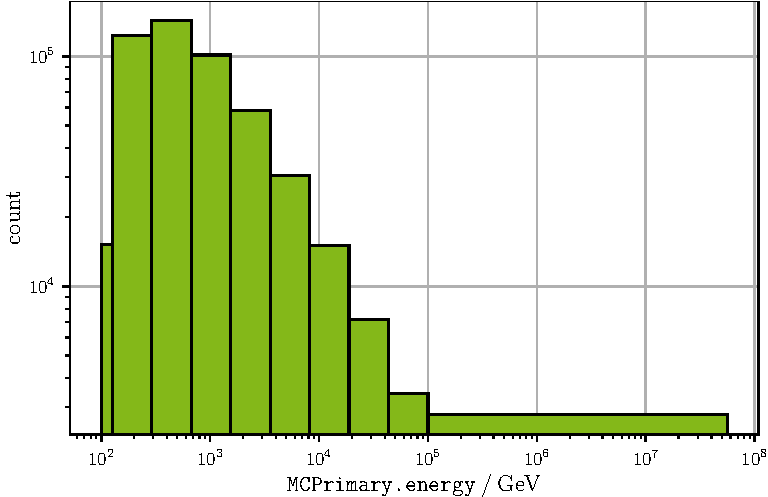
\includegraphics[scale=1]{content/plots/dataset_500k:discretized:histogram_full.pdf}
  \caption{Energy spectrum of the 500k Monte Carlo dataset using the discretized energy ranges as bins.}
  \label{fig:dataset:discretized:histogram}
\end{figure}


\subsection{Neural network}
A PyTorch \cite{pytorch} implementation of the \corn{} method
as well as several examples demonstrating its application on different datasets
is provided by \cite{corn}.
% TODO: Reference their tabular data / cement example?

This work makes use of said implementation of \corn{}
and hence the PyTorch framework.
Additionally,
  PyTorch Lightning \cite{pytorch_lightning},
  TorchMetrics \cite{torch_metrics}, % Oxford comma
  and scikit-learn \cite{sklearn}
  are used.

The neural network consists of \num{4} fully connected hidden layers.
The input layer has \num{12} neurons,
  corresponding to the number of features,
while the output layer has \num{9} neurons,
  corresponding to the number of binary classification subtasks,
    i.e. the number of bins minus one.
% \corn in the output layer…
% In total, the neural network has \num{TODO} neurons.

The number of neurons in the hidden layers is shown in \autoref{tab:nn_shape}.
\todo{Write a few sentences about these bullet points.}
\begin{itemize}
  \item Leaky ReLU activation function
  \item Fully connected layers
  \item Adam optimizer
\end{itemize}

\begin{table}
  \centering
  \begin{tabular}{S[table-format=3.0] c}
    \toprule
    {neurons} & {activation function} \\
    \midrule
    12  & – \\
    120 & leaky ReLU \\
    240 & leaky ReLU \\
    120 & leaky ReLU \\
    12  & leaky ReLU \\
    9   & leaky ReLU \\
    \bottomrule
  \end{tabular}
  % TODO: Ich habe immer gelernt: „Abbildungen haben eine Unterschrift, Tabellen eine Überschrift.“ @Karolin widerspricht dem scheinbar.
  \caption{
    Shape and activation functions of the neural network.
    The number of neurons in the input and output layers is determined by the number of features and bins, respectively.
  }
  \label{tab:nn_shape}
\end{table}

% TODO: Reference \corn loss function?

\textsc{Adam} (Adaptive Moment Estimation) \cite{adam} is used as the optimizer.
% It combines the benefits of both AdaGrad and RMSProp.

The neural network keeps its weights between \dsea{} iterations.
This was found to have no significant effect on the performance \cite{dsea_samuel}. % (\texttt{one\_model})


\subsection{DSEA}
For this work, the Python implementation of \dsea{} \cite{dsea_code} by \citeauthor{dsea_mirko} is used.
It expects a \emph{scikit-learn} classifier.
In order to interface with this library,
a wrapper class is implemented,
  which exposes a constructor as well as the needed methods
  \mintinline{python}{fit(X, y, sample_weight)} and
  \mintinline{python}{predict_proba(X)}.
